
Originally the package was structured around two classes, FDataGrid and
FDataBasis, designed for each of the main data representations of the data and
consisted of four modules with basic statistics, operations and methods to
perform kernel smoothing.

\begin{figure}[Map of scikit-fda]{FIG:SCIKITMAP}{Map of scikit-fda \cite{scikitfda}}
	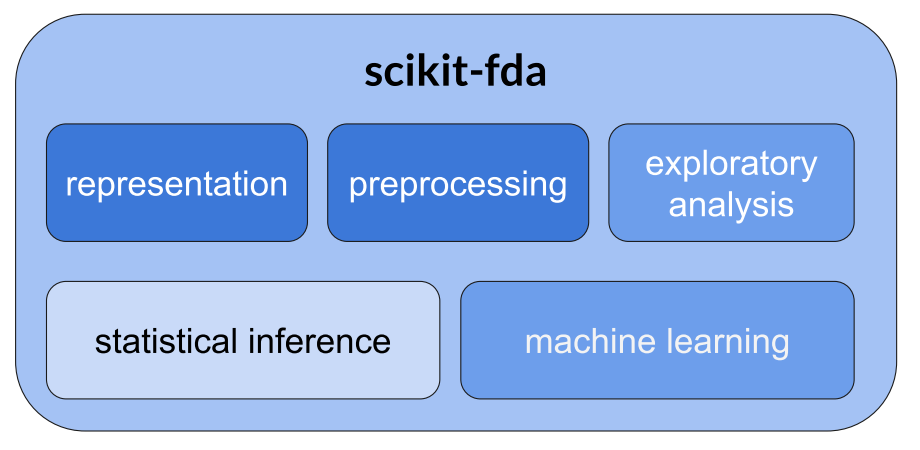
\includegraphics[width=10cm]{scikit-map}
\end{figure}


Due to the expansion of the project, the package has been completely
restructured, with a more hierarchical structure. Figure \ref{FIG:SCIKITMAP}
shows a diagram with a high-level description of this structure. The following
subsections summarize, in general terms, the functionalities incorporated and
design changes made during this work. A more detailed description may be found
in Annex \ref{CAP:GUIDE}, or in the documentation available \href{https://fda.readthedocs.io/en/latest/}{online}.

